In this section our main aim is to assign specified (previously bought) domain name to our .NET Core web application
as well as to configure SSL certificate for it.
What is domain name?
\begin{center}
    \textbf{Domain name} -- is a string of text that maps to a numeric IP address, used to access a website
    from client software~\cite{DomanNameCloudflare}.
    The actual address of a website is a complex numerical IP address (e.g.\ 103.21.244.0), but thanks to DNS,
    users are able to enter human-friendly domain names and be routed to the websites they are looking for.
\end{center}

\subsection{Buy and configure domain name using Cloudflare}\label{subsec:buy-and-configure-domain-name-using-cloudflare}
For instance, the domain name can be bought on the one of the following resources
\begin{itemize}
    \item \href{https://www.name.com/}{\texttt{https://www.name.com}}
    \item \href{https://www.namecheap.com/}{\texttt{https://www.namecheap.com}}
    \item \href{https://get.tech/}{\texttt{https://get.tech}}
\end{itemize}
After that we have to associate our domain with the \href{https://www.cloudflare.com/}{\texttt{cloudflare.com}} service in order
to manage out domain name and get some free DDoS protection and request analytics.
For instance, I have bought a domain name withing \href{https://www.name.com/}{\texttt{name.com}} service
and configured it using the following DNS records:
\begin{itemize}
    \item \texttt{hassan.ns.cloudflare.com}
    \item \texttt{sonia.ns.cloudflare.com}
\end{itemize}
So it looks like as follows
\begin{figure}[H]
    \centering
    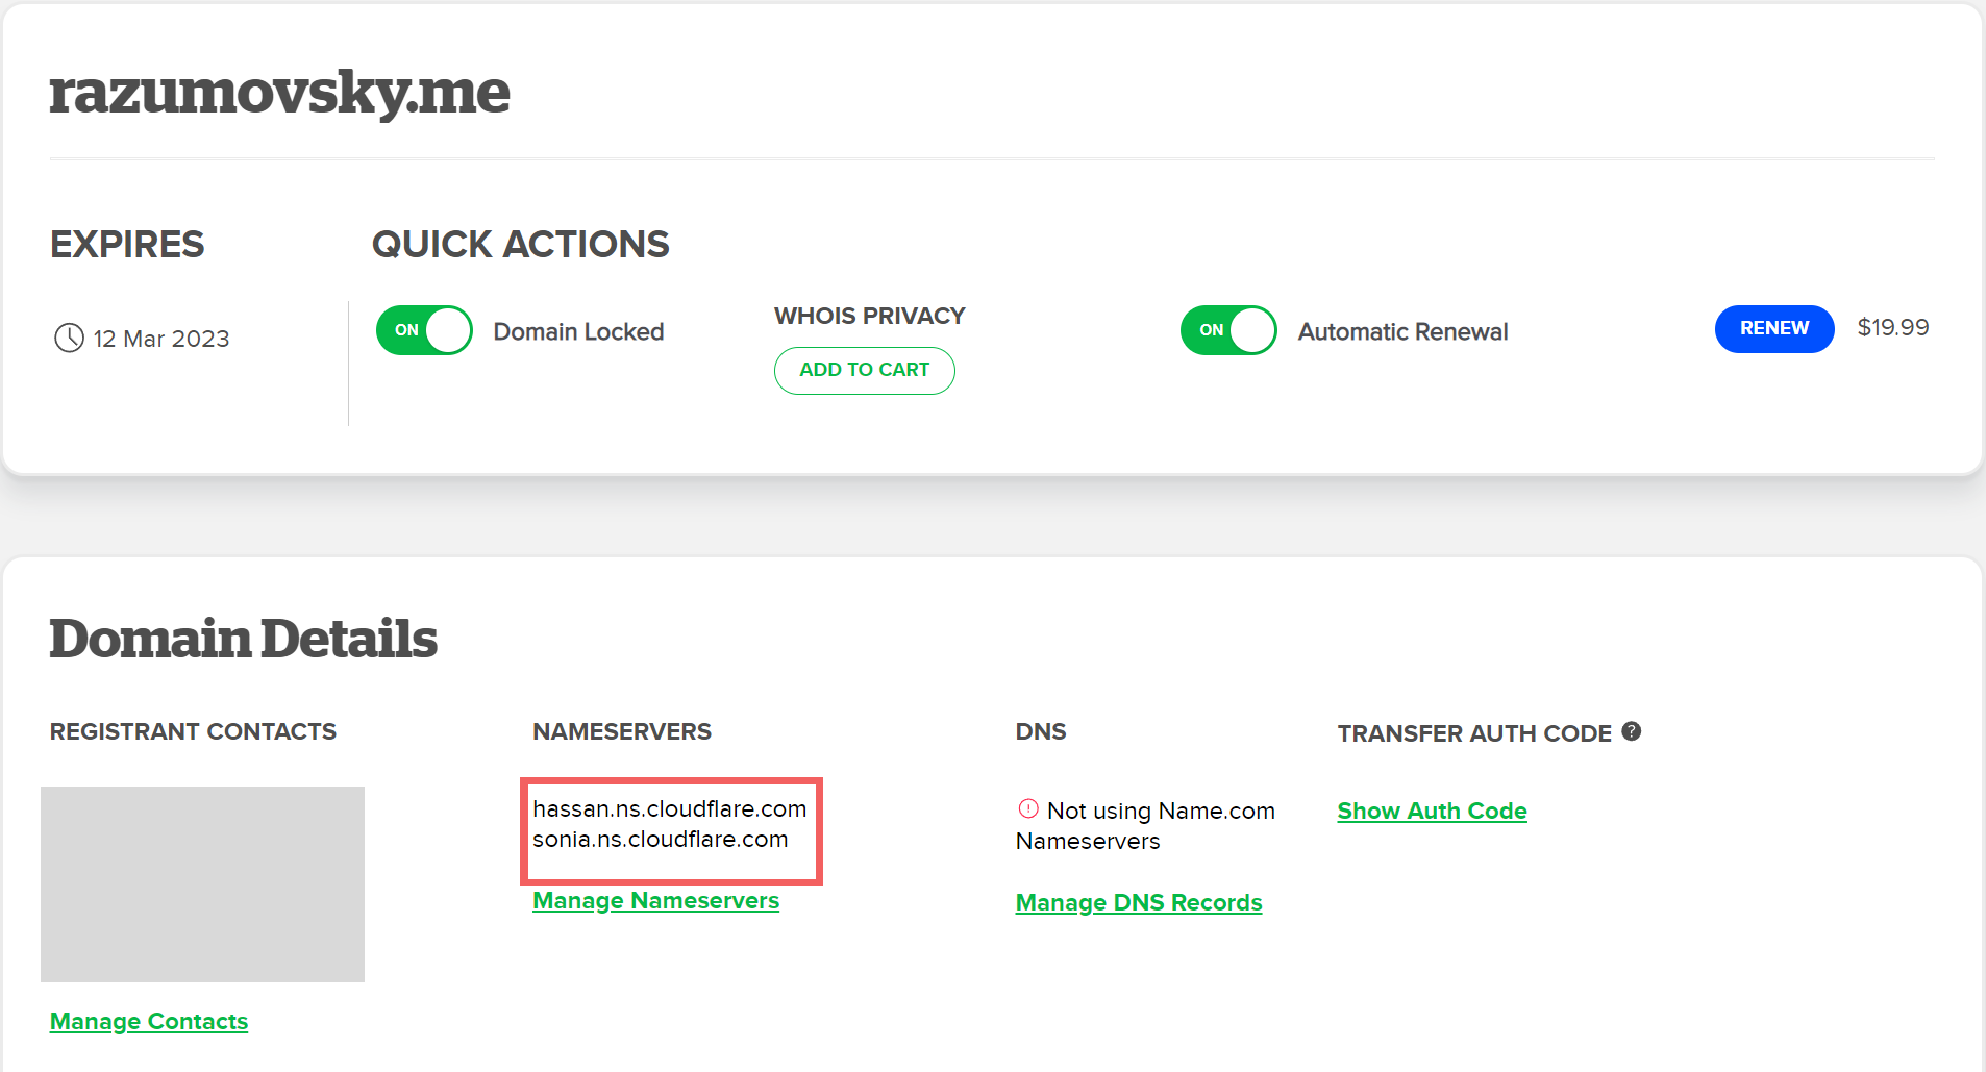
\includegraphics[width=1\textwidth]{img/07_domain_at_name_com}
    ~\caption{Domain name configuration at \href{https://www.name.com/}{\texttt{name.com}}.}\label{fig:figure18}
\end{figure}
After that we have to configure our domain name at cloudflare providing an IP address of the virtual machine we host
our .NET Core web application, that is
\begin{figure}[H]
    \centering
    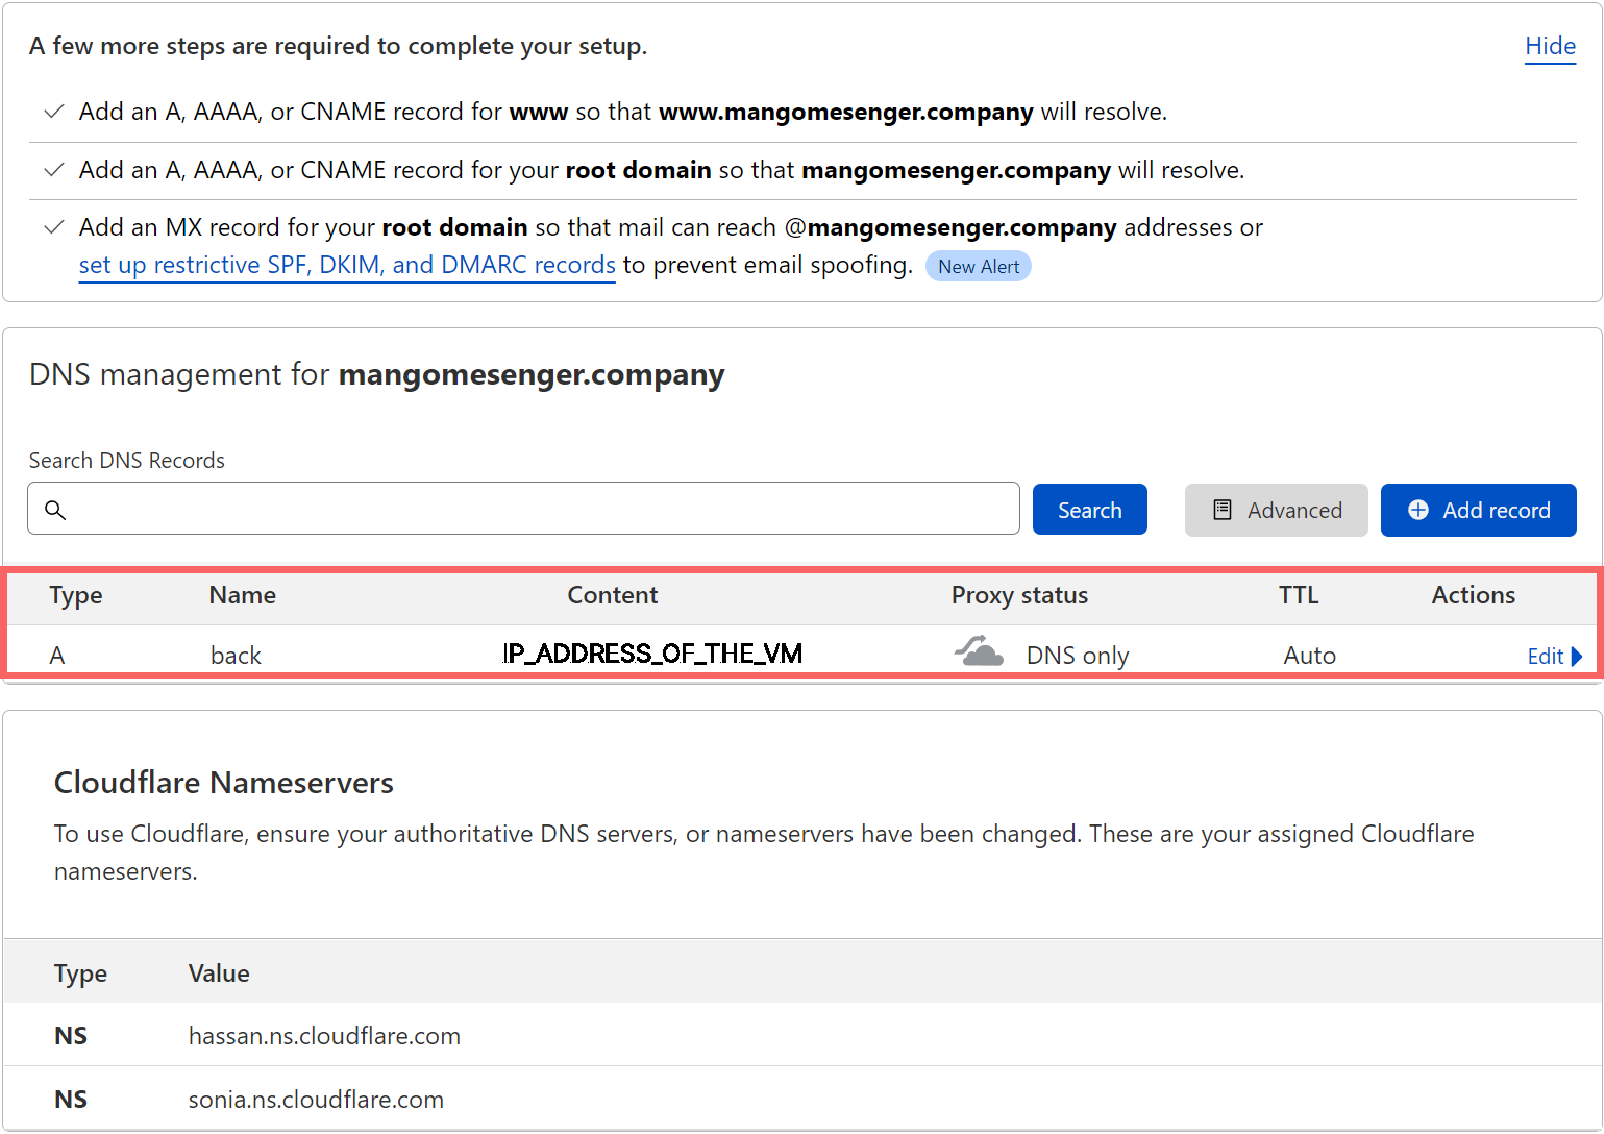
\includegraphics[width=1\textwidth]{img/07_domain_at_cloudflare_com}
    ~\caption{Domain name configuration at \href{https://www.cloudflare.com/}{\texttt{cloudflare.com}}.}\label{fig:figure19}
\end{figure}

\subsection{Configure nginx for the Domain name}\label{subsec:configure-nginx-for-the-domain-name}
Now our aim is to make sure that \texttt{nginx} server accepts connections to the VM via the Domain name we
previously bought and configured.
Yet again we use SSH + RSA key pair and change the address in our \texttt{nginx} configuration as follows
\begin{spverbatim}
    server {
        server_name back.mangomesenger.company;

        location / {
            include proxy_params;
            proxy_pass http://127.0.0.1:8080;
        }

        location /swagger {
            include proxy_params;
            proxy_pass http://127.0.0.1:8080;
        }

        location /api {
            include proxy_params;
            proxy_pass http://127.0.0.1:8080;
        }

        location /notify {
            proxy_pass http://127.0.0.1:8080;
            proxy_http_version 1.1;
            proxy_set_header Upgrade $http_upgrade;
            proxy_set_header Connection "upgrade";
            proxy_set_header Host $host;
            proxy_cache_bypass $http_upgrade;
        }
    }
\end{spverbatim}
We, actually, have changed only the top line \texttt{server\_name} to the
\begin{center}
    \texttt{server\_name back.mangomesenger.company;}
\end{center}
Let's restart and test the \texttt{nginx} server using the commands
\begin{itemize}
    \item \texttt{sudo systemctl restart nginx}
    \item \texttt{sudo nginx -t}
\end{itemize}
So that our web application is available now under the \texttt{HTTP} external url, yet without SSL certificate
\begin{center}
    \href{http://back.mangomesenger.company/swagger}{\texttt{http://back.mangomesenger.company/swagger}}
\end{center}
And it works as desired
\begin{figure}[H]
    \centering
    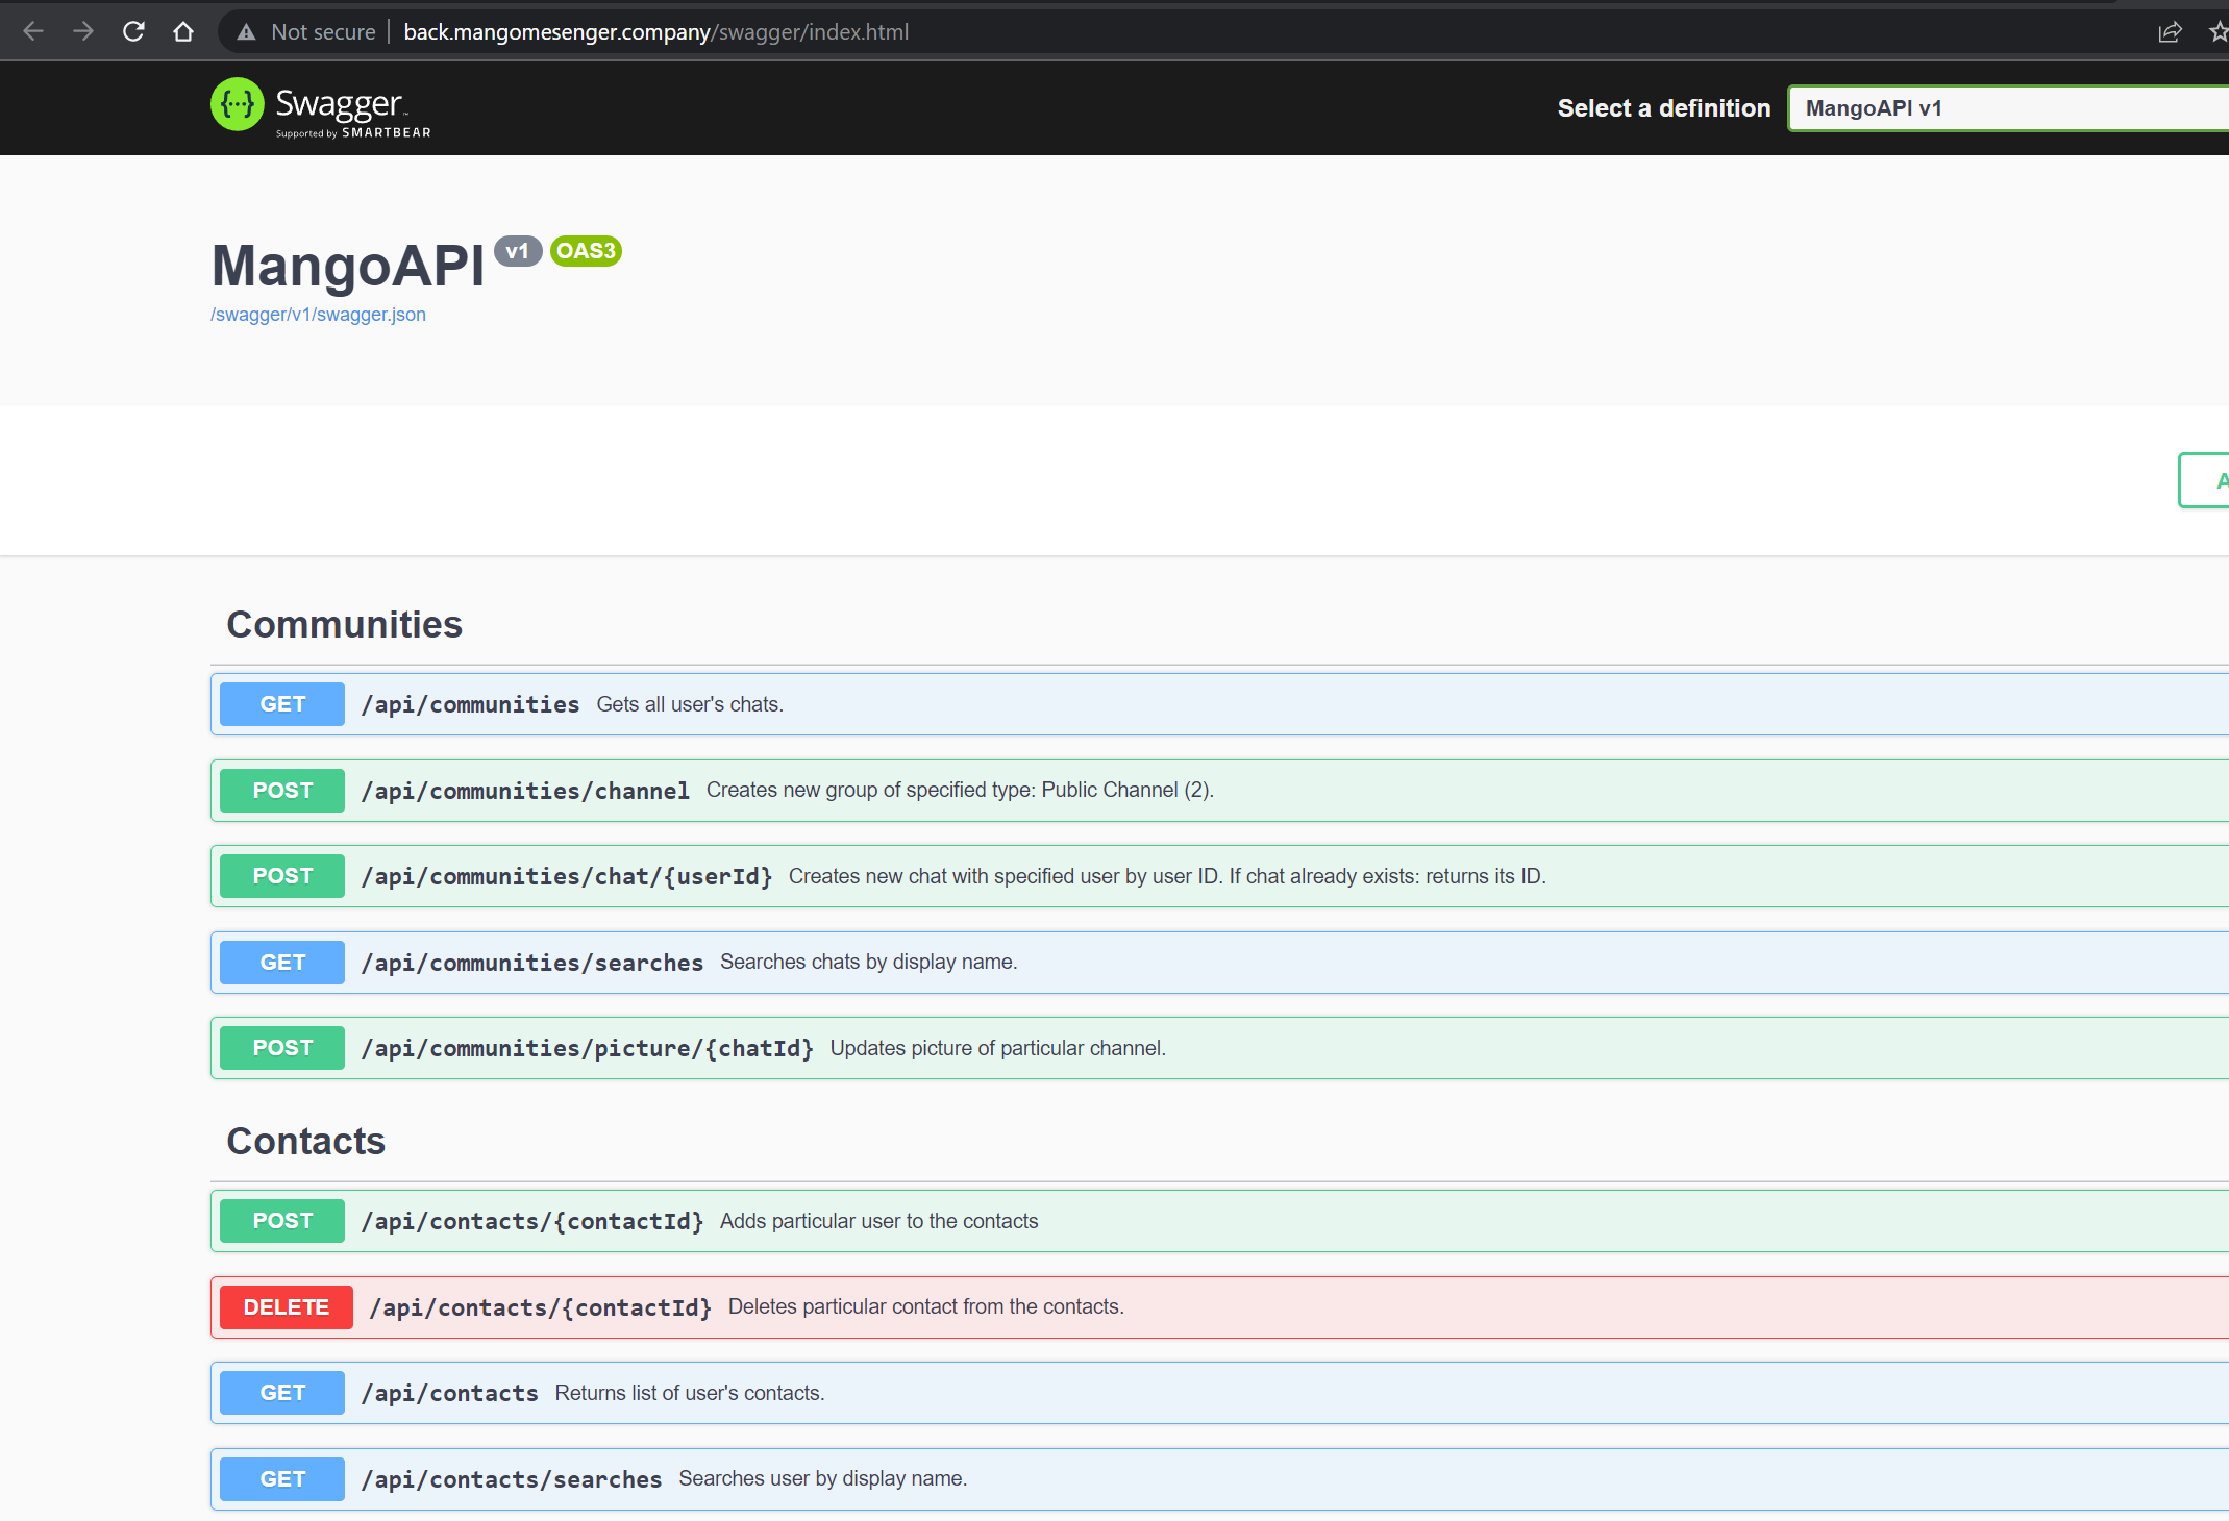
\includegraphics[width=1\textwidth]{img/07_swagger_under_domain_name}
    ~\caption{Application is available under the Domain name.}\label{fig:figure20}
\end{figure}

\subsection{Configure the HTTPS using LetsEncrypt Certbot}\label{subsec:configure-https-using-letsencrypt-certbot}
Configuring the \texttt{HTTPS} for our \texttt{nginx} server we are going to use the \texttt{CertBot} tool
from the \texttt{LetsEncrypt}.
We install it to the Ubuntu virtual machine using the following commands:
\begin{itemize}
    \item \texttt{sudo apt update -y}
    \item \texttt{sudo apt install -y python3 python3-pip python3-dev build-essential}
    \item \texttt{sudo pip3 install --upgrade pip}
    \item \texttt{sudo pip3 install certbot}
    \item \texttt{sudo pip3 install certbot-nginx}
\end{itemize}
A partial terminal output is as follows
\begin{figure}[H]
    \centering
    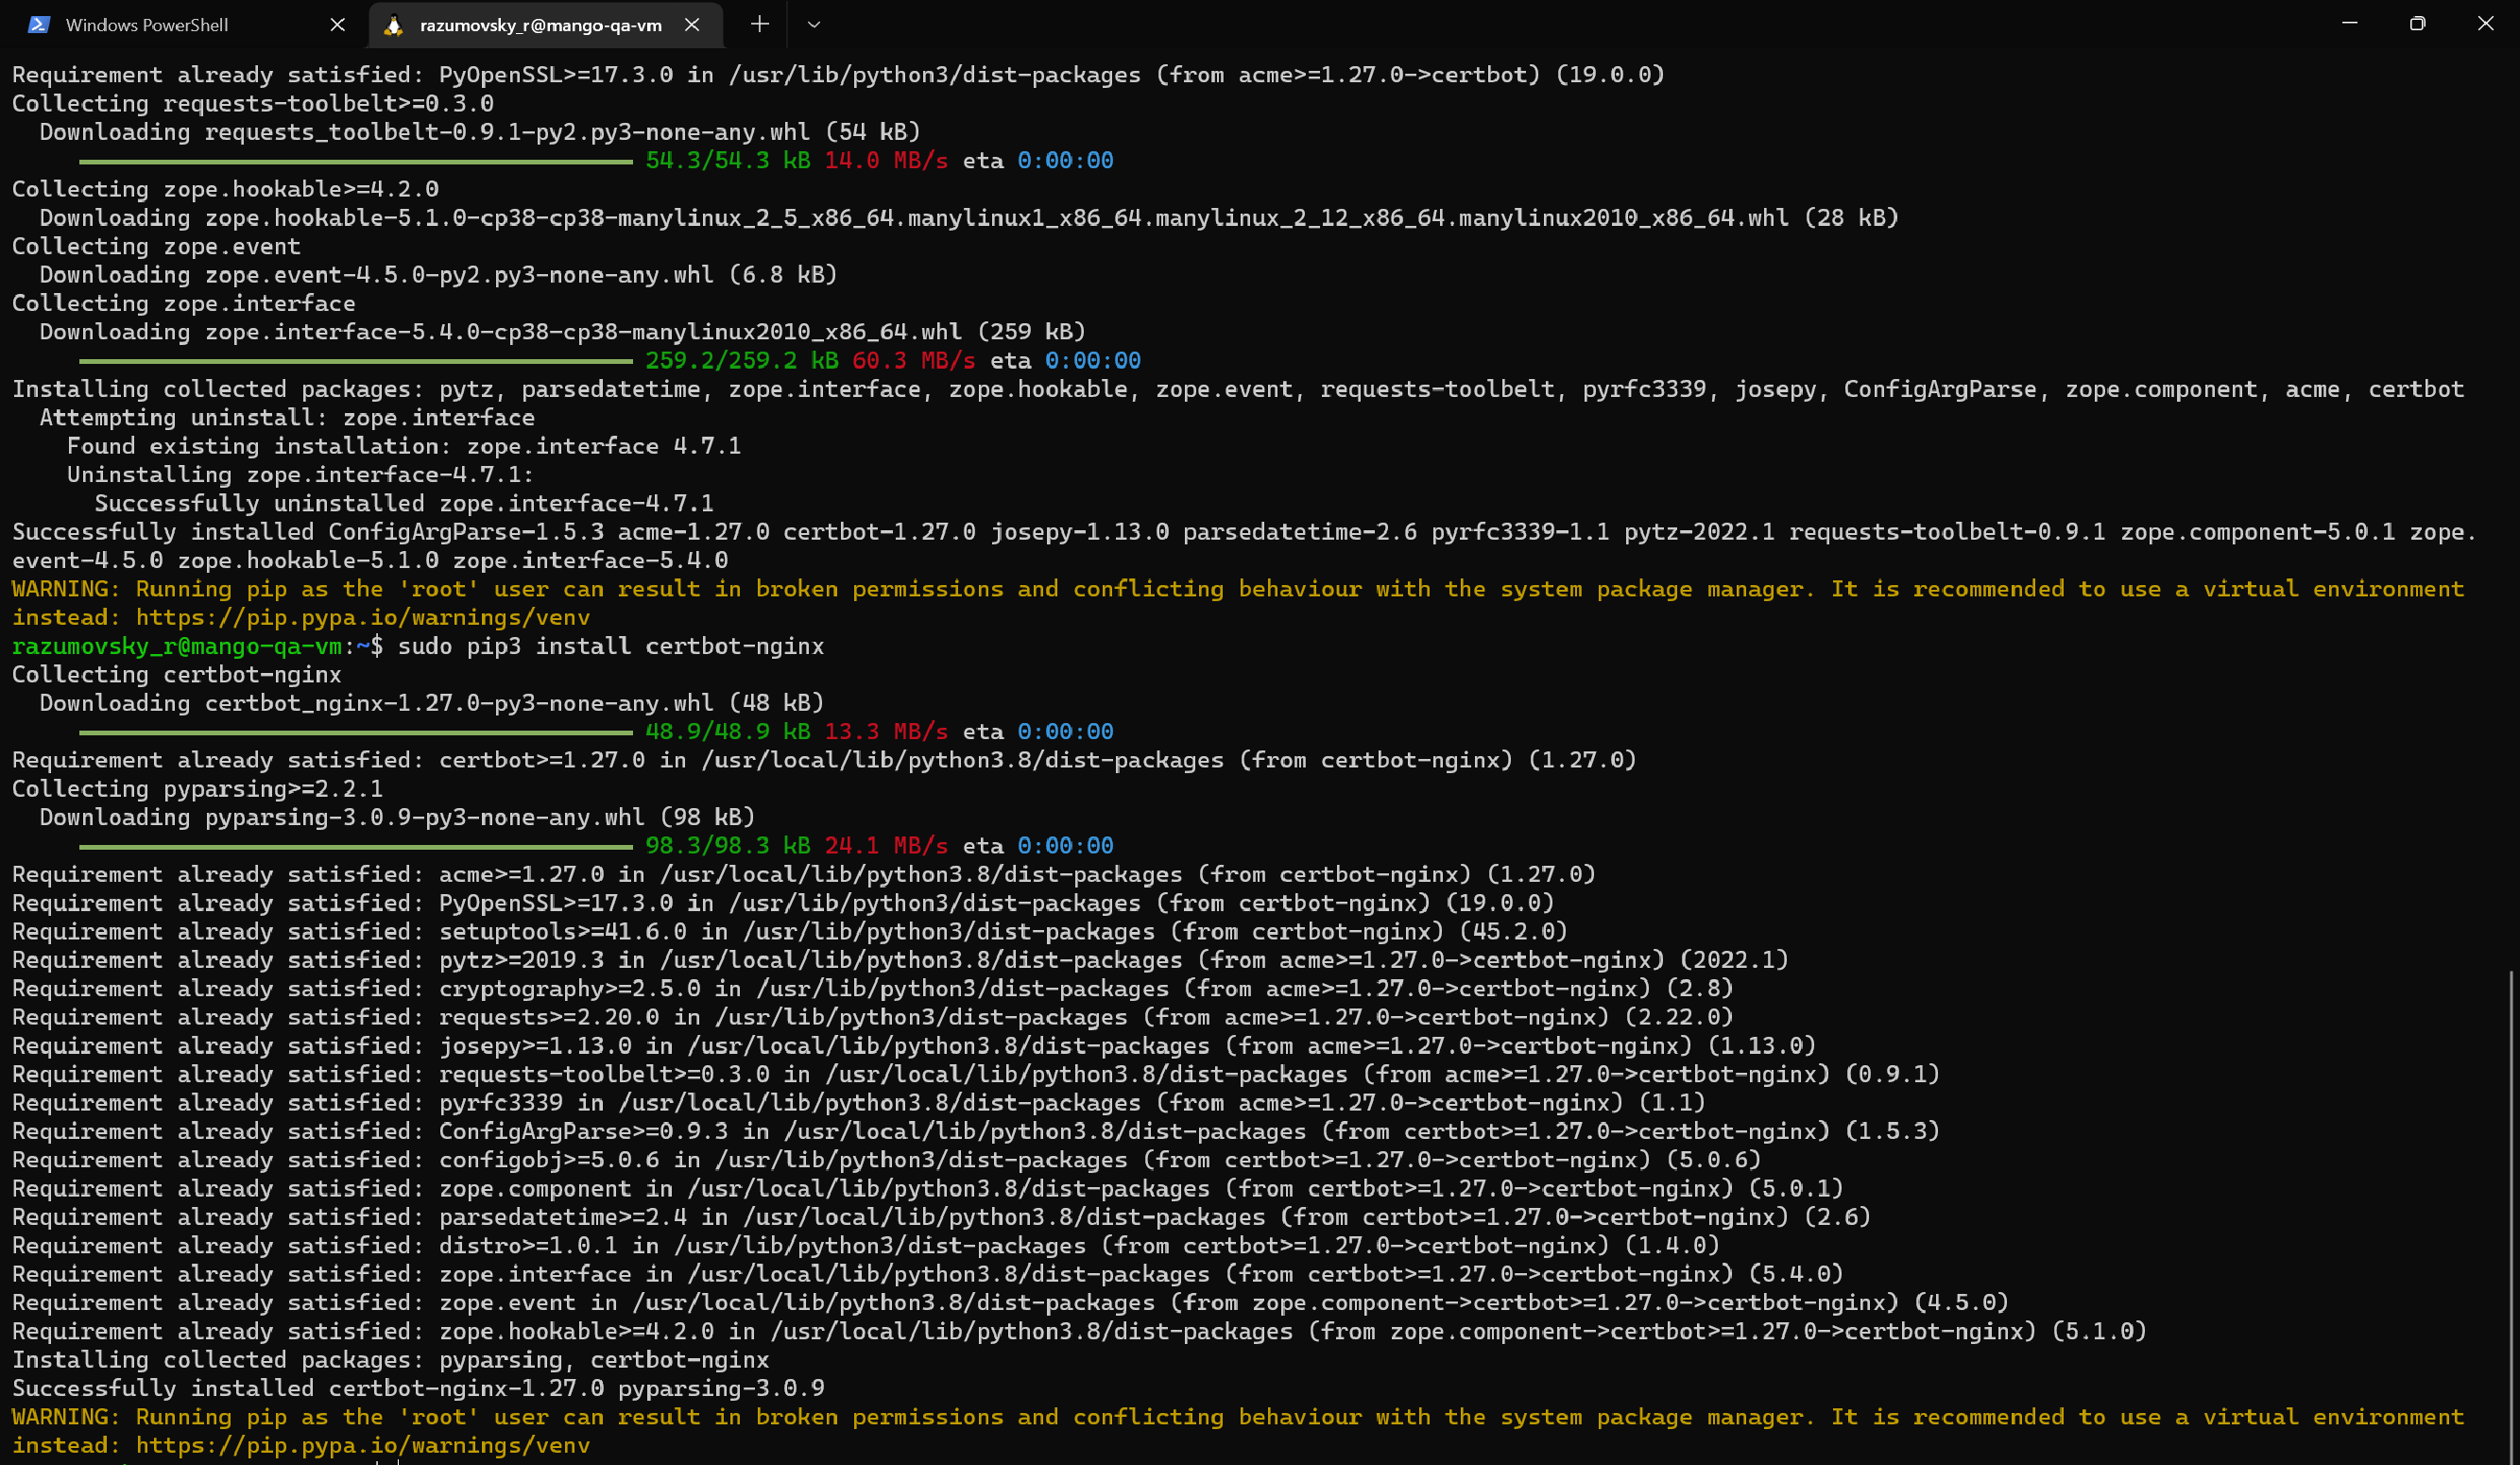
\includegraphics[width=1\textwidth]{img/07_install_certbot_console_output}
    ~\caption{Install \texttt{CertBot} tool terminal output.}\label{fig:figure21}
\end{figure}
Last part remaining is to certify out \texttt{nginx} web server so that it will accept \texttt{HTTPS} connections,
we do it using the commands:
\begin{itemize}
    \item \texttt{sudo certbot --nginx}
    \item \texttt{sudo systemctl restart nginx}
    \item \texttt{sudo nginx -t}
\end{itemize}
The terminal output is as follows
\begin{figure}[H]
    \centering
    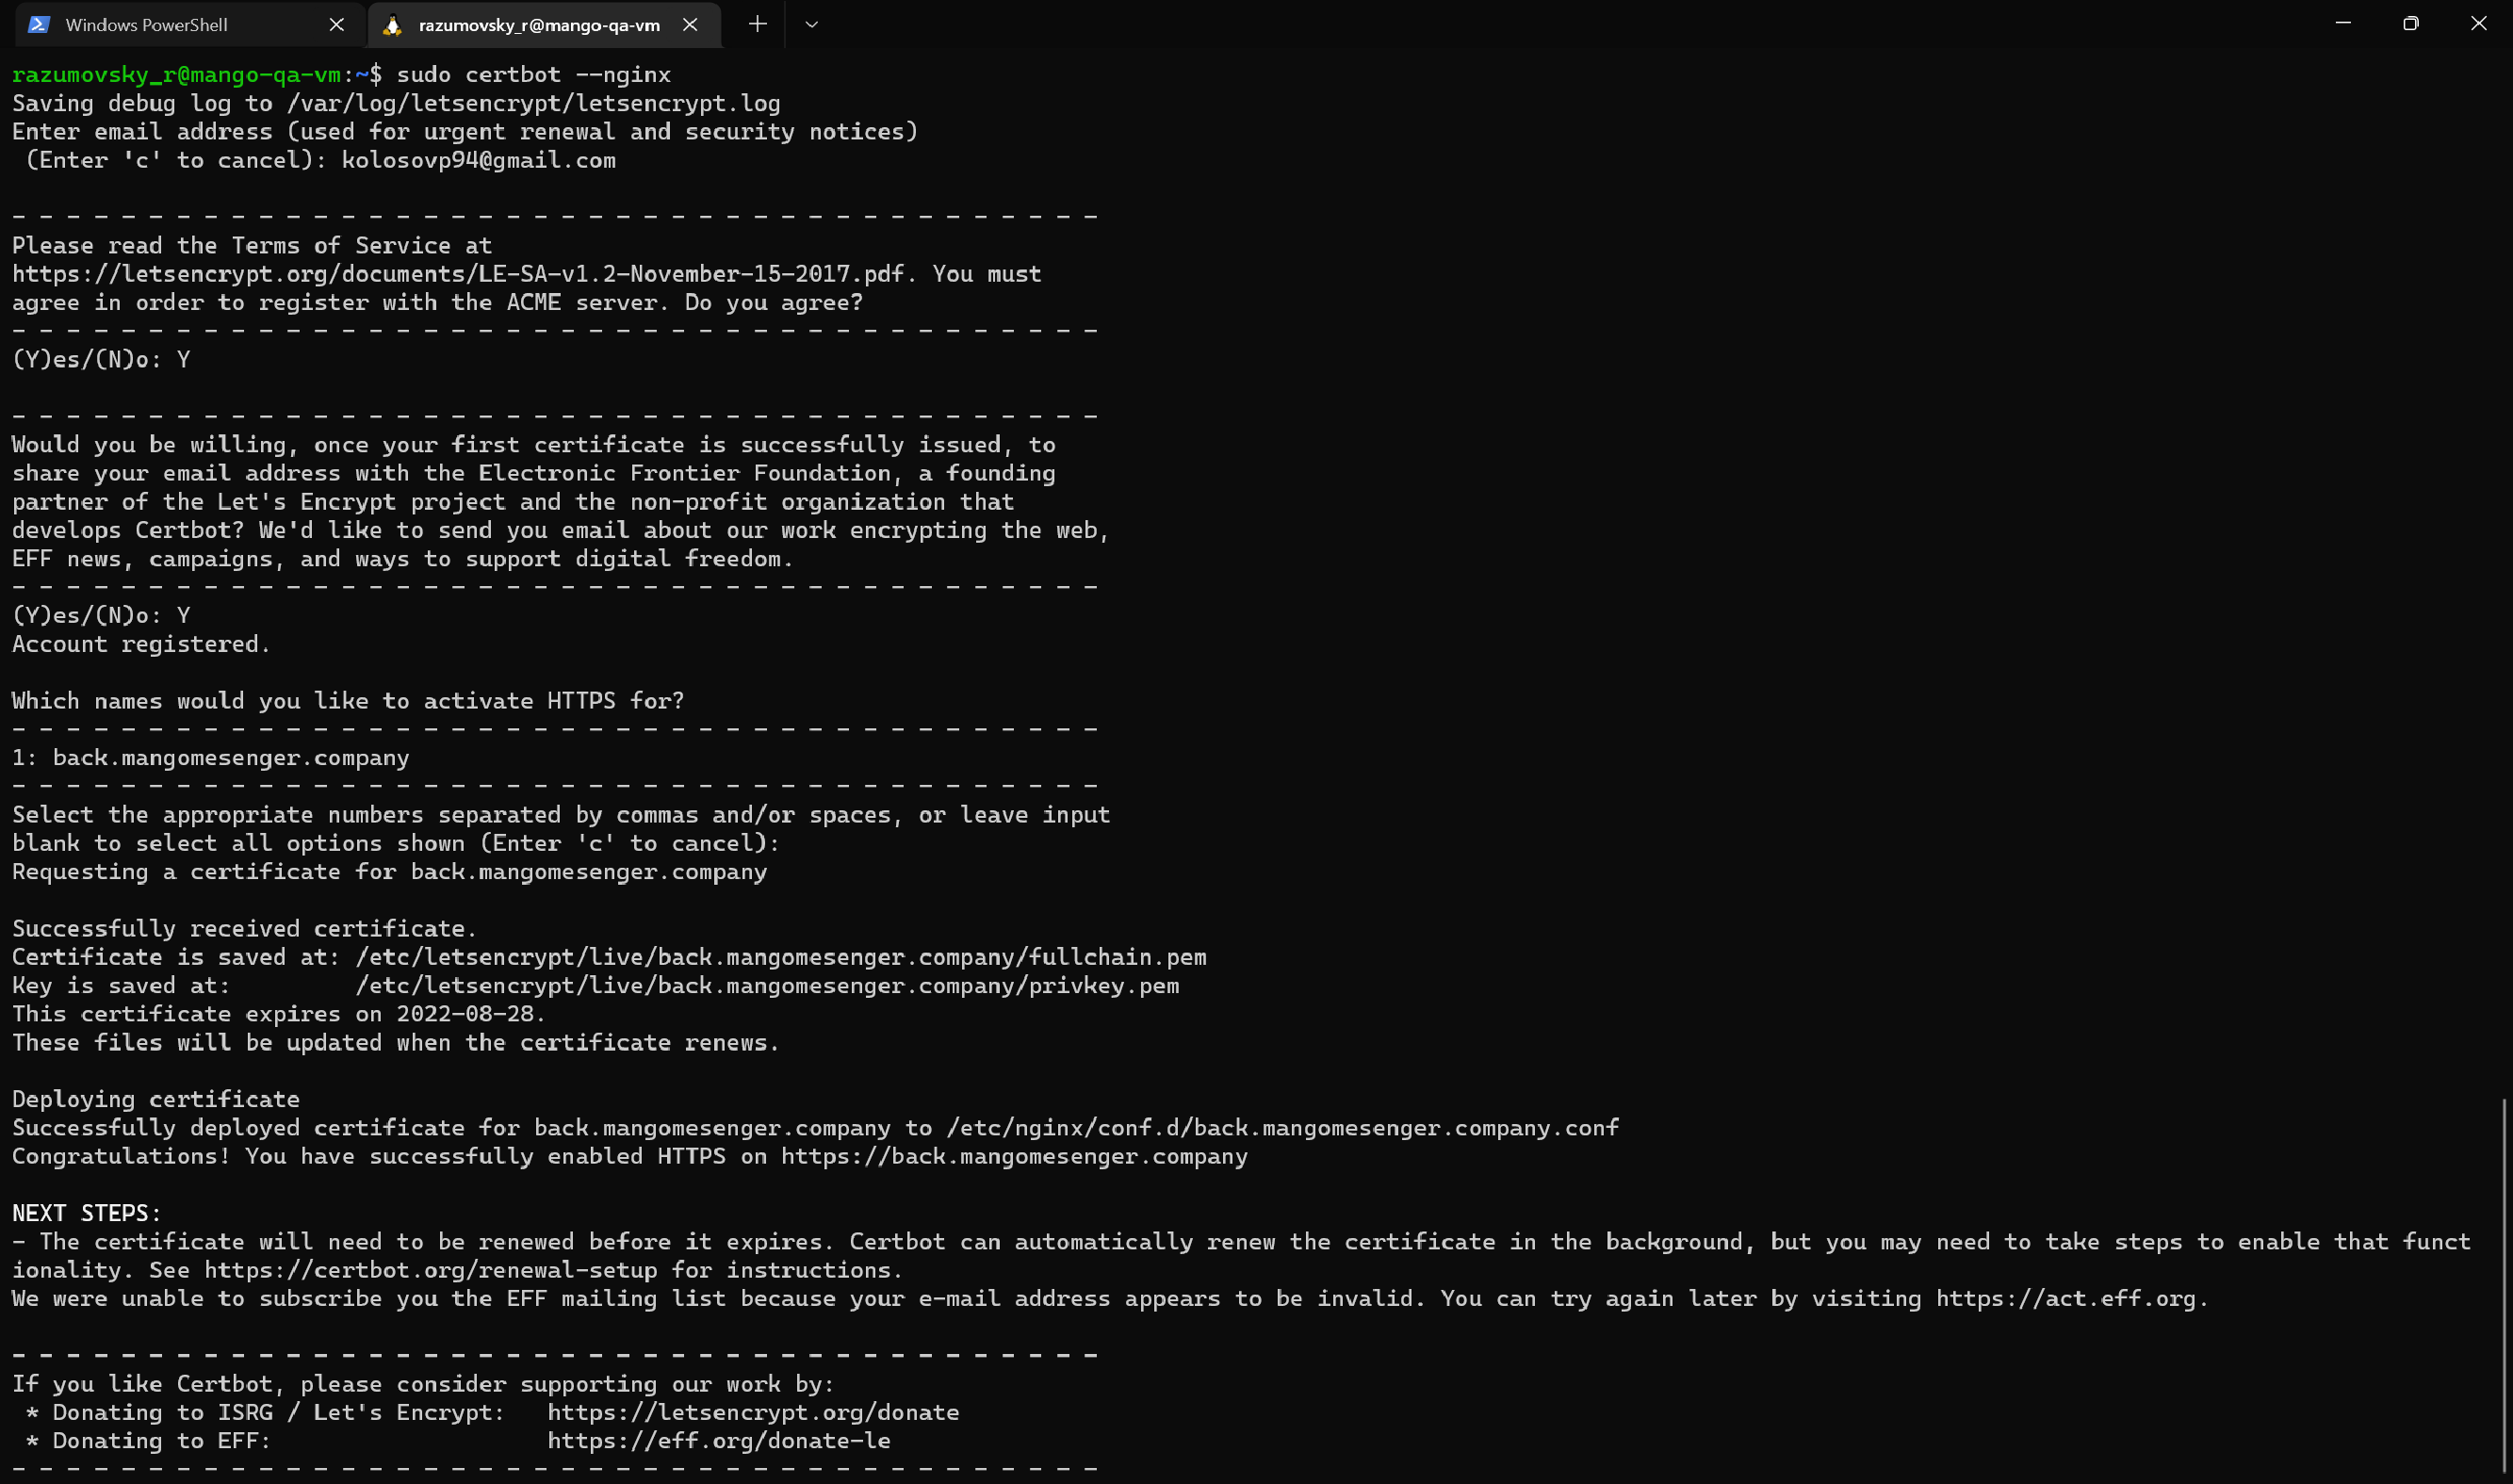
\includegraphics[width=1\textwidth]{img/07_certbot_nginx}
    ~\caption{\texttt{sudo certbot --nginx} terminal output.}\label{fig:figure22}
\end{figure}

Finally, our web application accepts the \texttt{HTTPS} connections now
\begin{center}
    \href{https://back.mangomesenger.company/swagger}{\texttt{https://back.mangomesenger.company/swagger}}
\end{center}
And certificate looks as follows
\begin{figure}[H]
    \centering
    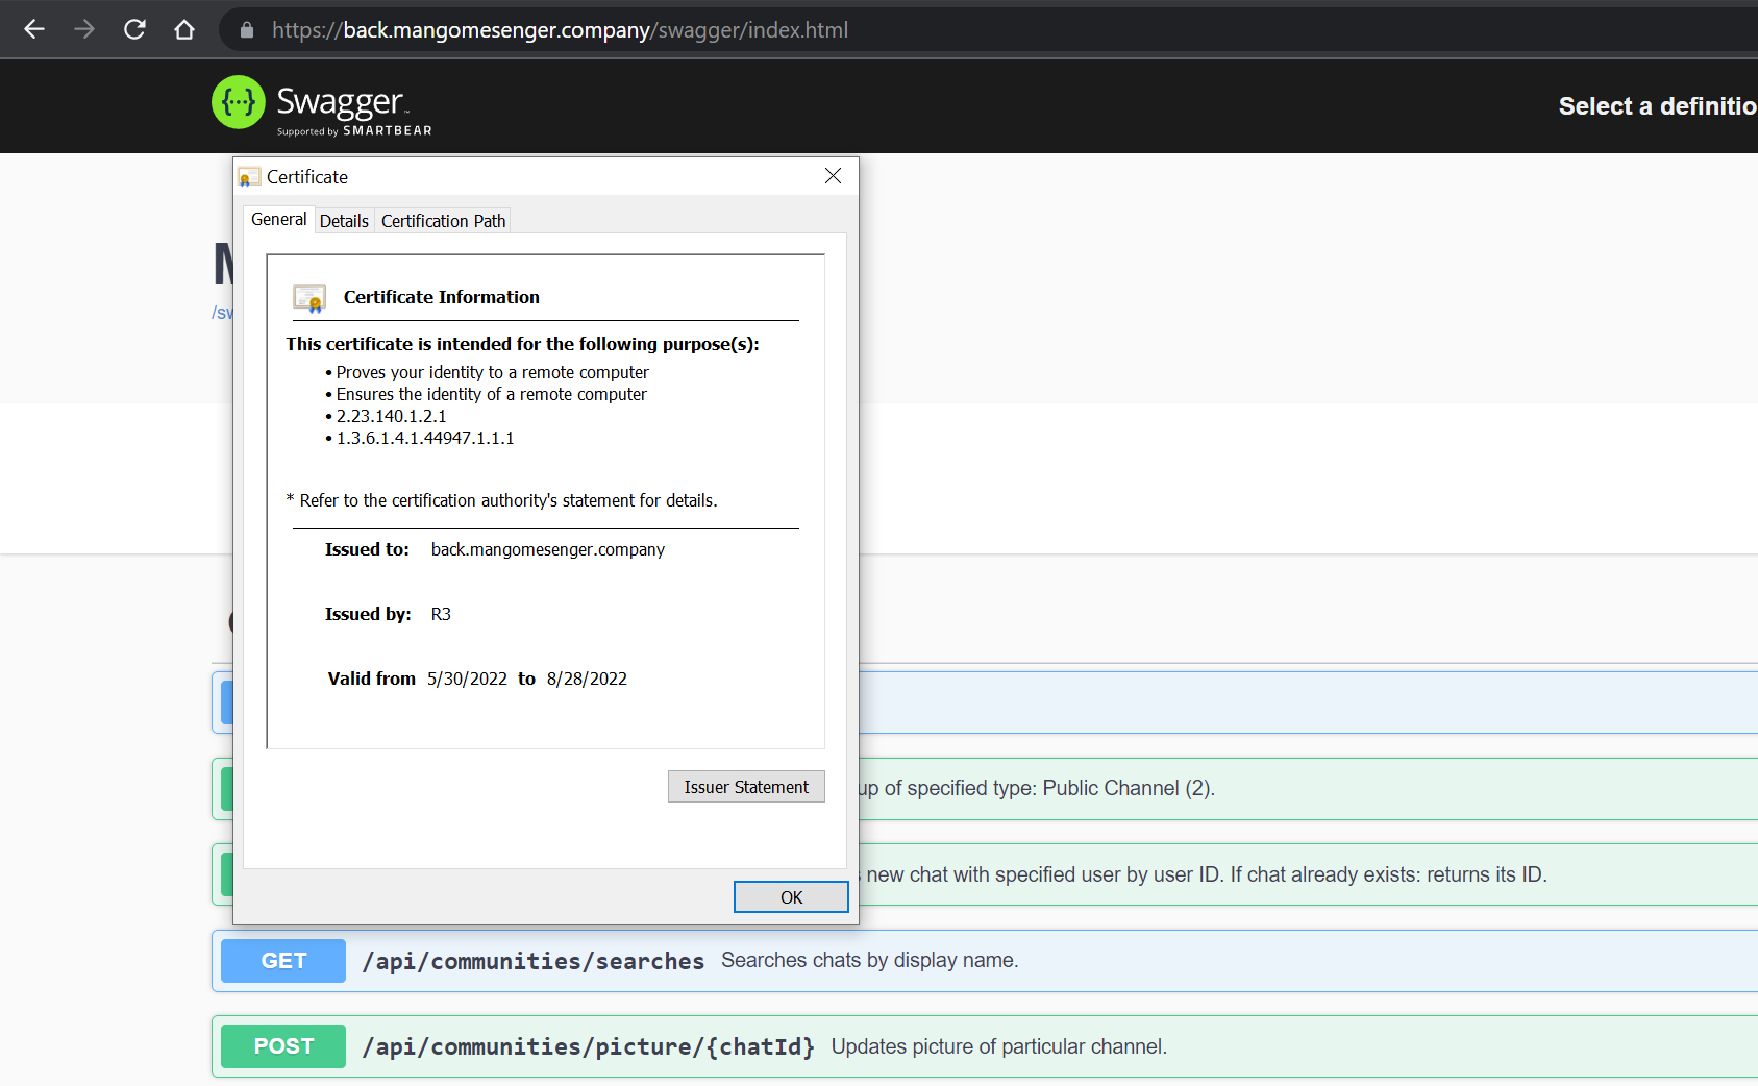
\includegraphics[width=1\textwidth]{img/07_https_browser_output}
    ~\caption{\texttt{sudo certbot --nginx} terminal output.}\label{fig:figure23}
\end{figure}
This completes the current section.